%% bare_conf.tex
%% V1.3
%% 2007/01/11
%% by Michael Shell
%% See:
%% http://www.michaelshell.org/
%% for current contact information.
%%
%% This is a skeleton file demonstrating the use of IEEEtran.cls
%% (requires IEEEtran.cls version 1.7 or later) with an IEEE conference paper.
%%
%% Support sites:
%% http://www.michaelshell.org/tex/ieeetran/
%% http://www.ctan.org/tex-archive/macros/latex/contrib/IEEEtran/
%% and
%% http://www.ieee.org/

%%*************************************************************************
%% Legal Notice:
%% This code is offered as-is without any warranty either expressed or
%% implied; without even the implied warranty of MERCHANTABILITY or
%% FITNESS FOR A PARTICULAR PURPOSE! 
%% User assumes all risk.
%% In no event shall IEEE or any contributor to this code be liable for
%% any damages or losses, including, but not limited to, incidental,
%% consequential, or any other damages, resulting from the use or misuse
%% of any information contained here.
%%
%% All comments are the opinions of their respective authors and are not
%% necessarily endorsed by the IEEE.
%%
%% This work is distributed under the LaTeX Project Public License (LPPL)
%% ( http://www.latex-project.org/ ) version 1.3, and may be freely used,
%% distributed and modified. A copy of the LPPL, version 1.3, is included
%% in the base LaTeX documentation of all distributions of LaTeX released
%% 2003/12/01 or later.
%% Retain all contribution notices and credits.
%% ** Modified files should be clearly indicated as such, including  **
%% ** renaming them and changing author support contact information. **
%%
%% File list of work: IEEEtran.cls, IEEEtran_HOWTO.pdf, bare_adv.tex,
%%                    bare_conf.tex, bare_jrnl.tex, bare_jrnl_compsoc.tex
%%*************************************************************************

% *** Authors should verify (and, if needed, correct) their LaTeX system  ***
% *** with the testflow diagnostic prior to trusting their LaTeX platform ***
% *** with production work. IEEE's font choices can trigger bugs that do  ***
% *** not appear when using other class files.                            ***
% The testflow support page is at:
% http://www.michaelshell.org/tex/testflow/



% Note that the a4paper option is mainly intended so that authors in
% countries using A4 can easily print to A4 and see how their papers will
% look in print - the typesetting of the document will not typically be
% affected with changes in paper size (but the bottom and side margins will).
% Use the testflow package mentioned above to verify correct handling of
% both paper sizes by the user's LaTeX system.
%
% Also note that the "draftcls" or "draftclsnofoot", not "draft", option
% should be used if it is desired that the figures are to be displayed in
% draft mode.
%
\documentclass[10pt, a4paper, onecolumn, conference, compsocconf]{IEEEtran}
% Add the compsocconf option for Computer Society conferences.
%
% If IEEEtran.cls has not been installed into the LaTeX system files,
% manually specify the path to it like:
% \documentclass[conference]{../sty/IEEEtran}





% Some very useful LaTeX packages include:
% (uncomment the ones you want to load)


% *** MISC UTILITY PACKAGES ***
%
\usepackage{ifpdf}
% Heiko Oberdiek's ifpdf.sty is very useful if you need conditional
% compilation based on whether the output is pdf or dvi.
% usage:
% \ifpdf
%   % pdf code
% \else
%   % dvi code
% \fi
% The latest version of ifpdf.sty can be obtained from:
% http://www.ctan.org/tex-archive/macros/latex/contrib/oberdiek/
% Also, note that IEEEtran.cls V1.7 and later provides a builtin
% \ifCLASSINFOpdf conditional that works the same way.
% When switching from latex to pdflatex and vice-versa, the compiler may
% have to be run twice to clear warning/error messages.






% *** CITATION PACKAGES ***
%
\usepackage{cite}
% cite.sty was written by Donald Arseneau
% V1.6 and later of IEEEtran pre-defines the format of the cite.sty package
% \cite{} output to follow that of IEEE. Loading the cite package will
% result in citation numbers being automatically sorted and properly
% "compressed/ranged". e.g., [1], [9], [2], [7], [5], [6] without using
% cite.sty will become [1], [2], [5]--[7], [9] using cite.sty. cite.sty's
% \cite will automatically add leading space, if needed. Use cite.sty's
% noadjust option (cite.sty V3.8 and later) if you want to turn this off.
% cite.sty is already installed on most LaTeX systems. Be sure and use
% version 4.0 (2003-05-27) and later if using hyperref.sty. cite.sty does
% not currently provide for hyperlinked citations.
% The latest version can be obtained at:
% http://www.ctan.org/tex-archive/macros/latex/contrib/cite/
% The documentation is contained in the cite.sty file itself.






% *** GRAPHICS RELATED PACKAGES ***
%
\ifCLASSINFOpdf
\usepackage[pdftex]{graphicx}
  % declare the path(s) where your graphic files are
  % \graphicspath{{../pdf/}{../jpeg/}}
  % and their extensions so you won't have to specify these with
  % every instance of \includegraphics
  % \DeclareGraphicsExtensions{.pdf,.jpeg,.png}
\else
  % or other class option (dvipsone, dvipdf, if not using dvips). graphicx
  % will default to the driver specified in the system graphics.cfg if no
  % driver is specified.
\usepackage[dvips]{graphicx}
  % declare the path(s) where your graphic files are
  % \graphicspath{{../eps/}}
  % and their extensions so you won't have to specify these with
  % every instance of \includegraphics
  % \DeclareGraphicsExtensions{.eps}
\fi
% graphicx was written by David Carlisle and Sebastian Rahtz. It is
% required if you want graphics, photos, etc. graphicx.sty is already
% installed on most LaTeX systems. The latest version and documentation can
% be obtained at: 
% http://www.ctan.org/tex-archive/macros/latex/required/graphics/
% Another good source of documentation is "Using Imported Graphics in
% LaTeX2e" by Keith Reckdahl which can be found as epslatex.ps or
% epslatex.pdf at: http://www.ctan.org/tex-archive/info/
%
% latex, and pdflatex in dvi mode, support graphics in encapsulated
% postscript (.eps) format. pdflatex in pdf mode supports graphics
% in .pdf, .jpeg, .png and .mps (metapost) formats. Users should ensure
% that all non-photo figures use a vector format (.eps, .pdf, .mps) and
% not a bitmapped formats (.jpeg, .png). IEEE frowns on bitmapped formats
% which can result in "jaggedy"/blurry rendering of lines and letters as
% well as large increases in file sizes.
%
% You can find documentation about the pdfTeX application at:
% http://www.tug.org/applications/pdftex





% *** MATH PACKAGES ***
%
%\usepackage[cmex10]{amsmath}
% A popular package from the American Mathematical Society that provides
% many useful and powerful commands for dealing with mathematics. If using
% it, be sure to load this package with the cmex10 option to ensure that
% only type 1 fonts will utilized at all point sizes. Without this option,
% it is possible that some math symbols, particularly those within
% footnotes, will be rendered in bitmap form which will result in a
% document that can not be IEEE Xplore compliant!
%
% Also, note that the amsmath package sets \interdisplaylinepenalty to 10000
% thus preventing page breaks from occurring within multiline equations. Use:
%\interdisplaylinepenalty=2500
% after loading amsmath to restore such page breaks as IEEEtran.cls normally
% does. amsmath.sty is already installed on most LaTeX systems. The latest
% version and documentation can be obtained at:
% http://www.ctan.org/tex-archive/macros/latex/required/amslatex/math/





% *** SPECIALIZED LIST PACKAGES ***
%
%\usepackage{algorithmic}
% algorithmic.sty was written by Peter Williams and Rogerio Brito.
% This package provides an algorithmic environment fo describing algorithms.
% You can use the algorithmic environment in-text or within a figure
% environment to provide for a floating algorithm. Do NOT use the algorithm
% floating environment provided by algorithm.sty (by the same authors) or
% algorithm2e.sty (by Christophe Fiorio) as IEEE does not use dedicated
% algorithm float types and packages that provide these will not provide
% correct IEEE style captions. The latest version and documentation of
% algorithmic.sty can be obtained at:
% http://www.ctan.org/tex-archive/macros/latex/contrib/algorithms/
% There is also a support site at:
% http://algorithms.berlios.de/index.html
% Also of interest may be the (relatively newer and more customizable)
% algorithmicx.sty package by Szasz Janos:
% http://www.ctan.org/tex-archive/macros/latex/contrib/algorithmicx/




% *** ALIGNMENT PACKAGES ***
%
%\usepackage{array}
% Frank Mittelbach's and David Carlisle's array.sty patches and improves
% the standard LaTeX2e array and tabular environments to provide better
% appearance and additional user controls. As the default LaTeX2e table
% generation code is lacking to the point of almost being broken with
% respect to the quality of the end results, all users are strongly
% advised to use an enhanced (at the very least that provided by array.sty)
% set of table tools. array.sty is already installed on most systems. The
% latest version and documentation can be obtained at:
% http://www.ctan.org/tex-archive/macros/latex/required/tools/


%\usepackage{mdwmath}
%\usepackage{mdwtab}
% Also highly recommended is Mark Wooding's extremely powerful MDW tools,
% especially mdwmath.sty and mdwtab.sty which are used to format equations
% and tables, respectively. The MDWtools set is already installed on most
% LaTeX systems. The lastest version and documentation is available at:
% http://www.ctan.org/tex-archive/macros/latex/contrib/mdwtools/


% IEEEtran contains the IEEEeqnarray family of commands that can be used to
% generate multiline equations as well as matrices, tables, etc., of high
% quality.


%\usepackage{eqparbox}
% Also of notable interest is Scott Pakin's eqparbox package for creating
% (automatically sized) equal width boxes - aka "natural width parboxes".
% Available at:
% http://www.ctan.org/tex-archive/macros/latex/contrib/eqparbox/





% *** SUBFIGURE PACKAGES ***
\usepackage[tight,footnotesize]{subfigure}
% subfigure.sty was written by Steven Douglas Cochran. This package makes it
% easy to put subfigures in your figures. e.g., "Figure 1a and 1b". For IEEE
% work, it is a good idea to load it with the tight package option to reduce
% the amount of white space around the subfigures. subfigure.sty is already
% installed on most LaTeX systems. The latest version and documentation can
% be obtained at:
% http://www.ctan.org/tex-archive/obsolete/macros/latex/contrib/subfigure/
% subfigure.sty has been superceeded by subfig.sty.



\usepackage[caption=false]{caption}
\usepackage[font=footnotesize]{subfig}
% subfig.sty, also written by Steven Douglas Cochran, is the modern
% replacement for subfigure.sty. However, subfig.sty requires and
% automatically loads Axel Sommerfeldt's caption.sty which will override
% IEEEtran.cls handling of captions and this will result in nonIEEE style
% figure/table captions. To prevent this problem, be sure and preload
% caption.sty with its "caption=false" package option. This is will preserve
% IEEEtran.cls handing of captions. Version 1.3 (2005/06/28) and later 
% (recommended due to many improvements over 1.2) of subfig.sty supports
% the caption=false option directly:
\usepackage[caption=false,font=footnotesize]{subfig}
%
% The latest version and documentation can be obtained at:
% http://www.ctan.org/tex-archive/macros/latex/contrib/subfig/
% The latest version and documentation of caption.sty can be obtained at:
% http://www.ctan.org/tex-archive/macros/latex/contrib/caption/
\usepackage[brazil]{babel}
\usepackage[utf8]{inputenc}


% *** FLOAT PACKAGES ***
%
%\usepackage{fixltx2e}
% fixltx2e, the successor to the earlier fix2col.sty, was written by
% Frank Mittelbach and David Carlisle. This package corrects a few problems
% in the LaTeX2e kernel, the most notable of which is that in current
% LaTeX2e releases, the ordering of single and double column floats is not
% guaranteed to be preserved. Thus, an unpatched LaTeX2e can allow a
% single column figure to be placed prior to an earlier double column
% figure. The latest version and documentation can be found at:
% http://www.ctan.org/tex-archive/macros/latex/base/



%\usepackage{stfloats}
% stfloats.sty was written by Sigitas Tolusis. This package gives LaTeX2e
% the ability to do double column floats at the bottom of the page as well
% as the top. (e.g., "\begin{figure*}[!b]" is not normally possible in
% LaTeX2e). It also provides a command:
%\fnbelowfloat
% to enable the placement of footnotes below bottom floats (the standard
% LaTeX2e kernel puts them above bottom floats). This is an invasive package
% which rewrites many portions of the LaTeX2e float routines. It may not work
% with other packages that modify the LaTeX2e float routines. The latest
% version and documentation can be obtained at:
% http://www.ctan.org/tex-archive/macros/latex/contrib/sttools/
% Documentation is contained in the stfloats.sty comments as well as in the
% presfull.pdf file. Do not use the stfloats baselinefloat ability as IEEE
% does not allow \baselineskip to stretch. Authors submitting work to the
% IEEE should note that IEEE rarely uses double column equations and
% that authors should try to avoid such use. Do not be tempted to use the
% cuted.sty or midfloat.sty packages (also by Sigitas Tolusis) as IEEE does
% not format its papers in such ways.





% *** PDF, URL AND HYPERLINK PACKAGES ***
%
%\usepackage{url}
% url.sty was written by Donald Arseneau. It provides better support for
% handling and breaking URLs. url.sty is already installed on most LaTeX
% systems. The latest version can be obtained at:
% http://www.ctan.org/tex-archive/macros/latex/contrib/misc/
% Read the url.sty source comments for usage information. Basically,
% \url{my_url_here}.





% *** Do not adjust lengths that control margins, column widths, etc. ***
% *** Do not use packages that alter fonts (such as pslatex).         ***
% There should be no need to do such things with IEEEtran.cls V1.6 and later.
% (Unless specifically asked to do so by the journal or conference you plan
% to submit to, of course. )


% correct bad hyphenation here
\hyphenation{op-tical net-works semi-conduc-tor}


\begin{document}
%
% paper title
% can use linebreaks \\ within to get better formatting as desired
\title{MobDatU: A New Model for Human Mobility Prediction\\ Based on Heterogeneous Data}


% author names and affiliations
% use a multiple column layout for up to two different
% affiliations

%\author{\IEEEauthorblockN{Authors Name/s per 1st Affiliation (Author)}
%\IEEEauthorblockA{line 1 (of Affiliation): dept. name of organization\\
%line 2: name of organization, acronyms acceptable\\
%line 3: City, Country\\
%line 4: Email: name@xyz.com}
%\and
%\IEEEauthorblockN{Authors Name/s per 2nd Affiliation (Author)}
%\IEEEauthorblockA{line 1 (of Affiliation): dept. name of organization\\
%line 2: name of organization, acronyms acceptable\\
%line 3: City, Country\\
%line 4: Email: name@xyz.com}
%}

%\author{\IEEEauthorblockN{Lucas Maia Silveira and Jussara M. Almeida}
%\IEEEauthorblockA{Universidade Federal de Minas Gerais\\ 
%UFMG\\
%Belo Horizonte, MG – Brasil\\
%\{lucasmsil,jussara\}@dcc.ufmg.br}
%\and
%\IEEEauthorblockN{Humberto Marques-Neto}
%\IEEEauthorblockA{Pontifícia Universidade Católica de Minas Gerais \\
%PUC MINAS\\
%Belo Horizonte, MG -- Brasil\\
%humberto@pucminas.br}
%\and
%\IEEEauthorblockN{Artur Ziviani}
%\IEEEauthorblockA{Laboratório Nacional de Computação Científica \\
%LNCC\\
%Petrópolis, RJ -- Brasil\\
%ziviani@lncc.br}
%}

\author{\IEEEauthorblockN{Lucas Maia Silveira\IEEEauthorrefmark{1},
Jussara M. Almeida\IEEEauthorrefmark{1},
Humberto Marques-Neto\IEEEauthorrefmark{2} and 
Artur Ziviani\IEEEauthorrefmark{3}}
\IEEEauthorblockA{\IEEEauthorrefmark{1}Universidade Federal de Minas Gerais (UFMG)\\
Belo Horizonte, MG – Brazil\\ Email: \{lucasmsil,jussara\}@dcc.ufmg.br}
\IEEEauthorblockA{\IEEEauthorrefmark{2}Pontifícia Universidade Católica de Minas Gerais (PUC MINAS)\\
Belo Horizonte, MG -- Brazil\\ Email: humberto@pucminas.br}
\IEEEauthorblockA{\IEEEauthorrefmark{3}Laboratório Nacional de Computação Científica (LNCC)\\
Petrópolis, RJ -- Brazil\\Email:ziviani@lncc.br}}


% conference papers do not typically use \thanks and this command
% is locked out in conference mode. If really needed, such as for
% the acknowledgment of grants, issue a \IEEEoverridecommandlockouts
% after \documentclass

% for over three affiliations, or if they all won't fit within the width
% of the page, use this alternative format:
% 
%\author{\IEEEauthorblockN{Michael Shell\IEEEauthorrefmark{1},
%Homer Simpson\IEEEauthorrefmark{2},
%James Kirk\IEEEauthorrefmark{3}, 
%Montgomery Scott\IEEEauthorrefmark{3} and
%Eldon Tyrell\IEEEauthorrefmark{4}}
%\IEEEauthorblockA{\IEEEauthorrefmark{1}School of Electrical and Computer Engineering\\
%Georgia Institute of Technology,
%Atlanta, Georgia 30332--0250\\ Email: see http://www.michaelshell.org/contact.html}
%\IEEEauthorblockA{\IEEEauthorrefmark{2}Twentieth Century Fox, Springfield, USA\\
%Email: homer@thesimpsons.com}
%\IEEEauthorblockA{\IEEEauthorrefmark{3}Starfleet Academy, San Francisco, California 96678-2391\\
%Telephone: (800) 555--1212, Fax: (888) 555--1212}
%\IEEEauthorblockA{\IEEEauthorrefmark{4}Tyrell Inc., 123 Replicant Street, Los Angeles, California 90210--4321}}




% use for special paper notices
%\IEEEspecialpapernotice{(Invited Paper)}




% make the title area
\maketitle
\def\abstractname{Abstract}
\begin{abstract}
Several previous mobility models aim at describing or predicting human behavior in a particular region during a certain period of time. Nevertheless, most of those models have been evaluated using data from a single source, such as data from mobile calls or GPS data obtained from Web applications. Thus, the effectiveness of such models when using different types of data remains unknown.  This paper proposes a new model to predict human mobility, called MobDatU, which was designed to use data from  mobile calls and data from georeferenced applications (in an isolated or combined way).  MobDatU  as well as   two state-of-the-art models, namely SMOOTH and Leap Graph, are evaluated considering various scenarios with single data source and multiple data sources. The experiments indicate that MobDatU always produces results that are better than or at least comparable to the best baseline in all scenarios,  unlike the previous models whose performance is very dependent  on the particular type of data used.
\end{abstract}
\def\abstractname{Resumo}
\begin{abstract}
Atualmente existem diversos modelos de mobilidade humana que visam descrever ou prever o comportamento humano em uma região durante um período de tempo. Entretanto, a maioria desses modelos foram avaliados utilizando dados de uma única fonte, por exemplo, dados de chamadas de telefonia móvel ou dados de GPS obtidos a partir de aplicações Web georreferenciadas. Portanto, a robustez destes modelos a diferentes tipos de dados é ainda desconhecida. Neste artigo, é proposto um novo modelo de previsão de mobilidade humana, chamado MobDatU, que foi projetado para utilizar tanto dados de telefonia móvel quanto dados de aplicativos georreferenciados (isolada e  conjuntamente). O  MobDatU, assim como  dois modelos  estado-da-arte, a saber SMOOTH e Leap Graph, são avaliados considerando  diversos cenários com  dados de fonte única e de múltiplas fontes. Os experimentos indicam que MobDatU atinge resultados melhores ou pelo menos comparáveis ao melhor modelo estado-da-arte em todos os cenários, diferentemente dos modelos alternativos cujo desempenho é bem mais sensível ao tipo de dado utilizado.
\end{abstract}


\begin{IEEEkeywords}
Human mobility; georeferenced applications; mobile technology
\end{IEEEkeywords}


% For peer review papers, you can put extra information on the cover
% page as needed:
% \ifCLASSOPTIONpeerreview
% \begin{center} \bfseries EDICS Category: 3-BBND \end{center}
% \fi
%
% For peerreview papers, this IEEEtran command inserts a page break and
% creates the second title. It will be ignored for other modes.
\IEEEpeerreviewmaketitle

%%%%%%%%%%%%%%%%%%%%%%%%%%%%%%%%%%%%%%%%%%%%%%%%%%%%%%%%%%%%%%

\section{Introdução}

O entendimento sobre a mobilidade humana pode ajudar governos e empresas a prever e planejar ações  para melhorar a qualidade de vida das pessoas de uma determinada região. Tais previsões e planejamentos de ações podem ser feitas a partir de modelos de previsão de mobilidade, que por sua vez podem ser desenvolvidos a partir da análise de dados sobre deslocamentos de pessoas. Esses dados podem ser provenientes de diferentes fontes, incluindo telefonia móvel \cite{barabasi2008} e aplicativos georreferenciados \cite{noulas2011}, como o Twitter.

Embora estudos recentes mostrem que a mobilidade humana em áreas urbanas possa ser bem previsível considerando rotinas diárias \cite{barabasi201002}, a vasta maioria dos modelos de previsão de mobilidade disponíveis na literatura \cite{Munjal2011, Dong2013, Kyunghan2012,allamanis2012} foi proposta ou pelo menos avaliada considerando uma única fonte de dados, tais como dados de chamadas de telefonia móvel ou dados coletados de aplicações Web georreferenciadas (\textit{e.g.}, Twitter). A robustez de tais modelos a dados de fontes diferentes é ainda desconhecida.   Mais ainda, o uso combinado de dados de diferentes fontes pode levar a previsões mais precisas ou à  cobertura de um maior volume da população. Entretanto,  a adequação e a eficácia dos modelos existentes a dados de múltiplas fontes também ainda são desconhecidas. 

Neste contexto, este trabalho apresenta um novo modelo de previsão de mobilidade humana, chamado MobDatU, que foi projetado para explorar dados de fontes heterogêneas, especificamente dados de telefonia móvel e dados de aplicações georreferenciadas. O MobDatU utiliza alguns princípios abordados em dois outros modelos considerados estado-da-arte, o Leap Graph \cite{Dong2013} e o SMOOTH \cite{Munjal2011}. Enquanto o Leap Graph foi avaliado com dados de telefonia móvel, tendo conseguido um taxa de acerto de 84\%  no estudo original, o SMOOTH foi anteriormente avaliado somente com dados de aplicativos georreferenciados. 


%Neste artigo, nós comparamos a eficácia da previsão dos três modelos em vários cenários consistindo de: (i) dados homogêneos provenientes de fonte única, sejam logs de chamadas de telefonia móvel, sejam dados de GPS coletados da aplicação Twitter; e (ii) dados heterogêneos a partir da combinação de ambas as fontes.  Os nossos resultados experimentais indicam que o novo modelo MobDatU alcança as maiores taxas de acerto em todos os cenários avaliados, tanto para os dados de telefonia móvel quanto para os dados do Twitter. Já o SMOOTH  atinge resultados comparáveis ao do nosso modelo quando dados de GPS são utilizados, mas tem desempenho muito inferior nos outros cenários. O Leap  Graph, por sua vez, obtém resultados similares ao do MobDatU para os cenários com dados de telefonia móvel (para os quais ele foi projetado) e também quando os dados das duas fontes são combinados. Entretanto, seu desempenho quando apenas dados  de GPS  são utilizados é inferior ao do SMOOTH e ao do MobDatU.

Neste artigo, nós comparamos a eficácia da previsão dos três modelos em vários cenários consistindo de: (i) dados homogêneos provenientes de fonte única, sejam logs de chamadas de telefonia móvel, sejam dados de GPS coletados da aplicação Twitter; e (ii) dados heterogêneos a partir da combinação de ambas as fontes.  Os nossos resultados experimentais indicam que o novo modelo MobDatU alcança as maiores taxas de acerto em todos os cenários avaliados. Já o SMOOTH  atinge resultados comparáveis ao do nosso modelo quando dados de GPS são utilizados, mas tem desempenho muito inferior nos outros cenários. O Leap  Graph, por sua vez, obtém resultados similares ao do MobDatU para os cenários com dados de telefonia móvel (para os quais ele foi projetado) e também quando os dados das duas fontes são combinados. Entretanto, seu desempenho quando apenas dados  de GPS  são utilizados é inferior ao do SMOOTH e ao do MobDatU. 



%Portanto, as contribuições deste artigo são: (i) a avaliação de dois modelos de previsão de mobilidade estado-da-arte, SMOOTH e Leap Graph, em diferentes cenários com dados homogêneos e heterogêneos; e (ii) a proposição de um novo modelo, MobDatU, que se mostra mais robusto do que os modelos de referência, já que obtêm resultados melhores ou pelo menos comparáveis ao melhor modelo em todos os cenários.

Portanto, as contribuições deste artigo são: (i) a avaliação de dois modelos de previsão de mobilidade estado-da-arte, SMOOTH e Leap Graph, em diferentes cenários com dados homogêneos e heterogêneos; e (ii) a proposição de um novo modelo, MobDatU, que produz resultados melhores ou pelo menos comparáveis ao melhor modelo tanto para os cenários de dados de telefonia móvel, quanto para os de Twitter.

O resto do artigo está organizado como segue. A Seção \ref{sec:trabalhos} discute a literatura sobre modelos de mobilidade humana. A Seção \ref{sec:modelos} formalmente apresenta a tarefa de previsão de mobilidade humana, explica o funcionamento dos dois modelos de referência e apresenta o novo modelo MobDatU. A metodologia de avaliação adotada, incluindo as coleções de dados utilizadas nos experimentos, é descrita na Seção \ref{sec:meth}, enquanto os resultados são discutidos na Seção \ref{sec:experimentos}. Conclusões e trabalhos futuros são apresentados na Seção \ref{sec:conclusao}.



%%%%%%%%%%%%%%%%%%%%%%%%%%%%%%%%%%%%%%%%%%%%%%%%%%%%%%%%%%%%%%

\section{Trabalhos Relacionados}\label{sec:trabalhos}


A literatura contém vários trabalhos que propõem modelos de previsão de mobilidade humana. Esses modelos utilizam diferentes tipos de dados e exploram diversas estratégias para tentar predizer com maior precisão a movimentação das pessoas (\textit{i.e.}, usuários) \cite{Bui2014}. Alguns destes modelos buscam prever as trajetórias das pessoas utilizando dados de GPS \cite{Zheng2011} ou dados de telefonia móvel \cite{Dong2013}. Outros  modelos realizam a previsão a partir de distribuições estatísticas que capturam padrões específicos identificados nos dados, tais como a  distribuição da distância percorrida por um usuário  \cite{Kyunghan2009, Rhee2008}.%, Munjal2011

De forma similar, outros trabalhos, como \cite{Hoyoung2008} e \cite{noulas2012}, exploram padrões diversos observados nos dados, tais como os lugares visitados pelas pessoas, a frequência de visitação e a regularidade dos padrões de locomoção de um usuário. Em \cite{noulas2011}, os autores exploram os locais visitados bem como as  distâncias de locomoção de um usuário dentro de uma mesma região  para prever sua localização em um momento futuro. Já em \cite{cho2011}, os autores abordam a previsão de mobilidade considerando tanto  trajetórias longas quanto trajetórias curtas.

Utilizando dados de GPS coletados de aplicações de redes sociais georreferenciadas, os modelos propostos em \cite{Musolesi2007} e \cite{Nguyen2012} exploram não somente os padrões de distância percorrida e locais visitados, mas também as relações de amizade  entre os usuários (inferidas a partir dos dados coletados). Ou seja, os modelos pressupõem que uma pessoa terá maior chance de ir para um local se um grande número de seus amigos frequentarem esse local. 

A previsão da mobilidade humana pode auxiliar na prevenção de doenças e desastres bem como no planejamento urbano. Por exemplo, os trabalhos de \cite{barabasi200806,Balcan2009} mostram que o conhecimento sobre a mobilidade das pessoas em uma determinada região pode auxiliar na tomada de  decisões  para melhor e mais rapidamente evitar a disseminação de uma doença, amenizar os danos causados por desastres e até mesmo evitar engarrafamentos durante as horas de pico. Além disso, tal conhecimento também pode auxiliar as operadoras a aperfeiçoarem seus serviços de telefonia móvel \cite{Xavier2012}.

Entretanto, os modelos de mobilidade humana disponíveis na literatura foram propostos ou avaliados considerando apenas uma fonte única de dados, sejam chamadas de telefonia móvel \cite{Dong2013,barabasi2008,Balcan2009}  sejam dados de GPS coletados de aplicações georreferenciadas \cite{Kyunghan2009, Rhee2008, Munjal2011, Musolesi2007, noulas2011, Nguyen2012, cho2011}. A robustez desses modelos a dados de fontes diversas, seja isolada ou conjuntamente, é o foco deste trabalho. Para tanto são selecionados dois modelos de referência, o SMOOTH \cite{Munjal2011} e o Leap Graph \cite{Dong2013}: enquanto o primeiro foi avaliado anteriormente somente a partir de dados de GPS, o segundo foi avaliado para dados de telefonia móvel.  Mais ainda, é proposto um novo modelo que herda princípios dos dois modelos de referência, mas é projetado para explorar dados de fontes heterogêneas. Os dois modelos de referência, bem como o novo modelo proposto, chamado MobDatU, são descritos na próxima seção. 


 

%%%%%%%%%%%%%%%%%%%%%%%%%%%%%%%%%%%%%%%%%%%%%%%%%%%%%%%%%%%%%%

\section{Modelos de Mobilidade}\label{sec:modelos}

Esta seção primeiramente apresenta formalmente a tarefa de previsão de mobilidade humana abordada neste artigo (Seção \ref{subsec:modelagem}). A seguir, ela descreve brevemente o funcionamento dos dois modelos de referência, SMOOTH e Leap Graph (Seção \ref{subsub:modelos}) e introduz o novo modelo de previsão proposto, o MobDatU (Seção \ref{subsec:mobdatu}).


\subsection{Previsão de Mobilidade Humana}\label{subsec:modelagem}

A tarefa de previsão de mobilidade abordada neste artigo pode ser definida como segue. Sejam uma área  alvo $R$, consistindo de um conjunto de regiões $r_i \in R$, um conjunto de usuários $u_i \in U$ e um intervalo de tempo $t \in \{0..T\}$ minutos. Sejam ainda um conjunto de treino $\mathcal{D}$ e um conjunto de teste $\mathcal{T}$, consistindo de tuplas $<u_i, r_i, t>$ que indicam que $u_i$ estava na região $r_i$ em $t$. Deseja-se construir um modelo para prever em que região $r_i$ um dado usuário $u_i$ estará em um dado momento $t$ utilizando apenas os dados de treino $\mathcal{D}$. Deseja-se ainda avaliar o modelo utilizando os dados de teste, ou seja,  utilizar o modelo desenvolvido para prever a localização (\textit{i.e.}, região) $r_i$ para cada tupla $<u_i, ? , t>$ no conjunto de teste $\mathcal{T}$.  

Note que a definição das regiões $r_i$ pode ser feita de diversas maneiras. Por exemplo, cada região pode ser definida por um ponto central $x_i,y_i$ (e.g, as coordenadas de uma estação rádio-base para o caso de dados de telefonia móvel)  e um raio $d$. Alternativamente, cada região pode  representar uma área quadrada com centro $x_i,y_i$ e lado $d$ (área total $d^2$).  A definição das regiões adotada por cada modelo é explicitada nas seções seguintes.  Note também que, neste trabalho,  o intervalo de tempo total $T$ é discretizado em janelas consecutivas $\Delta t$ para fins de computação dos deslocamentos dos usuários. Em outras palavras,  a localização de um usuário é predita considerando a granularidade de tempo de $\Delta t$ minutos.


A divisão dos dados disponíveis em treino e teste também pode ser feita de forma diversa, dependendo da disponibilidade dos dados. Entretanto, tal divisão deve  respeitar restrições temporais, ou seja, os dados de treino devem preceder os dados de teste (\textit{i.e.}, $\forall$ $<$$*,*,t_i$$>$ $\in$ $\mathcal{D}$  and  $\forall$ $<$*,*,$t_j$$>$ $\in \mathcal{T}$, $t_i$ $<$ $t_j$). Mais ainda, considerando que os padrões de mobilidade humana variam ao longo do dia ou mesmo em dias diferentes (\textit{e.g.}, dias de semana e fim de semana) \cite{Xavier2012},  é desejado que os dados de treino tenham sido obtidos em períodos comparáveis com aqueles do conjunto de teste. Por exemplo, se deseja prever a localização de usuários entre 8 e 9 da manhã, deve-se utilizar dados coletados do mesmo período em dias anteriores, ou dados coletados em um período imediatamente anterior. A definição dos conjuntos de treino e teste em nossos experimentos será discutida na Seção \ref{sec:dados}.



\subsection{Modelos de Referência}\label{subsub:modelos}

Esta seção descreve os principais componentes dos dois modelos de referência adotados neste trabalho, o SMOOTH \cite{Munjal2011} e o Leap Graph \cite{Dong2013}. Em nossos experimentos, nós utilizamos as implementações de ambos os modelos disponibilizadas pelos autores.\footnote{toilers.mines.edu e www.cs.utexas.edu/~wdong86/.} 
 
\subsubsection{SMOOTH}\label{subsub:smooth}

O modelo SMOOTH, proposto por \cite{Munjal2011}, captura a locomoção de um grupo de usuários $U$ em uma área bidimensional simulada, composta por um conjunto de regiões de interesse. Cada região $r_i$ é definida por coordenadas $x_i, y_i$ dentro da área simulada e  probabilidades $p_i$ de um usuário se deslocar para cada uma delas. A probabilidade $p_i$ portanto captura a popularidade da região $r_i$, isto é, o número esperado de pessoas que visitam $r_i$.  

A ideia básica do SMOOTH é simular a locomoção dos usuários $U$ utilizando cada probabilidade $p_i$ de forma interativa, onde cada passo representa uma janela de tempo $\Delta t$ minutos. Em cada passo, o modelo simula a locomoção de cada usuário $u_i \in U$  a partir de duas distribuições específicas extraídas do conjunto de treino: a distribuição das distâncias percorridas $f_{dist}$  e a distribuição dos tempos de pausa $f_{pausa}$.  Como em \cite{Munjal2011}, observamos que tais distribuições seguem leis de potência para todos os cenários simulados. Tais distribuições são caracterizadas pelo  parâmetro  $\alpha$ e por valores mínimo ($min$) e máximo ($max$)\footnote{Distribuição Acumulada Complementar dada por $f(x) = \frac{(x*max^\alpha - x*min^\alpha -max^\alpha)}{(x*max^\alpha)*(x*min^\alpha)}^{-\alpha}$. }.    

Em cada passo,  para cada usuário que não está em pausa (explicado posteriormente), primeiramente é computada a direção de deslocamento  em função da sua localização atual  e das probabilidades associadas a cada região $r_i \in R$.  Em seguida,  é selecionada aleatoriamente uma distância de deslocamento utilizando $f_{dist}$, e o deslocamento é simulado. Por fim, é escolhido aleatoriamente um tempo de pausa utilizando $f_{pausa}$. O usuário permanecerá neste local durante o intervalo de tempo $f_{pausa}$ selecionado. 

Conforme proposto em \cite{Munjal2011},  a cada usuário é associado um raio de cobertura $d$ que definirá a região na qual o usuário se encontra em cada passo de execução do modelo. Quando o usuário para em um ponto ($x_i,y_i$), é verificado se ele se encontra a uma distância $d$ de pelo menos uma região (ou seja, se ele cobre uma região). O usuário é associado à  região mais próxima coberta por ele. Caso ele não cubra nenhuma região, é introduzida uma nova região $r_i$ em $R$ definida pela sua localização atual. Ao final de cada passo, as probabilidades  associadas a cada região (inclusive as novas) são recomputadas. 

Logo, o  treinamento do modelo consiste em  extrair as distribuições $f_{dist}$ e $f_{pausa}$ bem como as regiões $r_i \in R$  do conjunto $\mathcal{D}$. Todas as regiões que aparecem no conjunto de treinamento são inicialmente introduzidas no conjunto $R$ com as probabilidades correspondentes.  Estas probabilidades são utilizadas para determinar as localizações iniciais dos usuários para a fase de simulação  dos deslocamentos, durante a qual são aprendidas novas regiões visitadas e suas probabilidades.

Durante a fase de teste,  os deslocamentos dos usuários do conjunto $\mathcal{T}$ são simulados utilizando o modelo aprendido, mantendo o conjunto $R$ fixo e considerando a localização inicial de cada usuário dada pela sua primeira aparição em $\mathcal{T}$.  As regiões visitadas pelos usuários durante a simulação são comparadas com os demais dados do conjunto  $\mathcal{T}$ para avaliar a precisão do modelo. 


\subsubsection{Leap Graph}\label{subsub:leap}

Em \cite{Dong2013}, os autores investigaram como utilizar dados de telefonia móvel para prever a mobilidade de usuários. 
Estes dados tipicamente correspondem a um conjunto de chamadas telefônicas. A cada chamada estão associados um identificador único do usuário, os instantes de início e fim da chamada, bem como as coordenadas (latitude e longitude) das antenas onde a chamada foi iniciada e finalizada e as identificações  dos setores utilizados nestas antenas\footnote{Cada antena é dividida em 3 setores de $120^{o}$, cada um responsável por cerca de um terço da área de cobertura da antena.}. 

No modelo proposto em \cite{Dong2013}, chamado Leap Graph, cada região $r_i \in R$  corresponde a uma antena, sendo definida pelas suas coordenadas e por um  raio $d$ que representa sua área de cobertura. Assim, uma chamada do usuário $u_i$ associada à  antena correspondente à região $r_i$ em um instante $t$ indica a presença de $u_i$ naquela região na janela de tempo que inclui $t$. O modelo tenta inferir os deslocamentos de cada usuário a partir de um grafo que captura a trajetória do usuário entre as regiões de $R$. 

A fase de treinamento, portanto consiste  primeiramente em criar um grafo de trajetórias para cada usuário  a partir dos dados em $\mathcal{D}$. No grafo $G_i$ criado para o usuário $u_i$,   cada vértice corresponde a uma região. Uma aresta entre $r_i$ e $r_j$ é adicionada toda vez que: (i) $u_i$ fez uma chamada que foi iniciada em $r_i$ e finalizada em $r_j$; ou (ii)  $u_i$ fez duas chamadas consecutivas, a primeira em $r_i$ e a segunda em $r_j$. 

Como proposto originalmente, o Leap Graph objetiva prever a próxima região em que um usuário estará dado a sua localização atual. Portanto, ele não considera a dimensão tempo e explora apenas as transições entre antenas feitas por cada usuário.  Para torná-lo comparável ao SMOOTH e ao MobDatU (que consideram o tempo)  e aplicá-lo à  tarefa de predição alvo,  nós adicionamos laços (arestas da região $r_i$ para ela mesma) para capturar os períodos entre chamadas consecutivas de um mesmo usuário, quando sua localização é desconhecida. Durante tais períodos, foi assumido que o usuário permaneceu a metade do tempo em uma região e a metade seguinte na outra. Ou seja, dadas duas chamadas consecutivas nas regiões $r_i$ e $r_j$ nos tempos $t_1$ e $t_2$ e considerando a discretização do tempo em janelas de duração $\Delta t$, foi computado o número  $w$ de janelas entre $t_1$ e $t_2$. Foram então adicionados laços em $r_i$ e $r_j$, cada um com peso $w/2$. 

Os grafos criados são então combinados em um grafo único ponderado $G$ que representa os deslocamentos  da população de usuários em $\mathcal{D}$. Para tal, os grafos de usuários $G_i$ são ordenados pelo instante da primeira chamada de cada usuário em $\mathcal{D}$ e processados conforme esta ordem. As arestas de todos os grafos são combinadas em $G$, sendo que o peso de uma aresta corresponde ao número de grafos de usuários em que ela aparece. Porém, para trajetórias cobrindo $n$ ou mais arestas que aparecem em múltiplos grafos, são considerados apenas a trajetória e os trechos que a sucedem  no primeiro grafo processado.  Em outras palavras, suponha que o grafo $G_1$ contenha a trajetória $\{r_1,r_2,r_3,r_4\}$ e que  grafo $G_2$ contenha a trajetória $\{r_1, r_2, r_3, r_5\}$.  Para $n=2$, o  grafo $G$ conterá as arestas $\{r_1, r_2, r_3, r_4\}$,  todas com peso 1, já que a trajetória $\{r_1,r_2,r_3\}$ ($n=2$ arestas) aparece nos dois grafos. Conforme os autores, esta medida é tomada para evitar contabilizar duplamente as mesmas trajetórias.  Ao final da combinação, os pesos de todas as arestas são normalizadas de forma que os pesos de todas as arestas de saída de cada vértice $r_i$ totalizem 1. 

A aplicação do modelo Leap Graph, durante a fase de teste, consiste em simular o grafo $G$ produzido durante o treinamento como uma cadeia de Markov. Para cada usuário, a sua posição inicial  é extraída da sua primeira chamada no conjunto $\mathcal{T}$ e que corresponde a um estado da cadeia.   A cadeia é então simulada para inferir a posição do usuário em sucessivos passos.  Em nossos experimentos, utilizamos $n=2$ pois esta escolha levou aos melhores resultados em \cite{Dong2013}. 



\subsection{MobDatU: Um Novo Modelo de Predição de Mobilidade Humana}\label{subsec:mobdatu}

%Definicao da tarefa
% Ideia basica de funcioamento do modelo
% Treinamento
% Teste
%Enfatizar diferencas dos baselines
O novo modelo MobDatU tem como objetivo explorar dados de fontes heterogêneas para capturar a movimentação dos usuários entre as regiões de $R$. A área total simulada pelo modelo é divida em regiões quadrangulares não sobrepostas $r_i$ (como em um {\it grid}). Cada região $r_i$ é definida por um centro $x_i,y_i$ e um  lado $d$\footnote{O  modelo também foi executado utilizando regiões circulares de raio $d$, apresentando resultados similares aos reportados neste artigo.}.

O MobDatU herda alguns aspectos dos dois modelos de referência. Por exemplo, assim como no SMOOTH, a cada região $r_i$ é associada uma  medida de popularidade, que, no MobDatU, representa o número de usuários que visitou  $r_{i}$ no conjunto de treino $\mathcal{D}$ (podendo ser 0).  
De forma similar ao Leap Graph (e diferentemente do SMOOTH), o MobDatU simula a movimentação dos usuários entre as regiões a partir de um grafo de transições. Entretanto, diferentemente do Leap Graph,  a criação deste grafo não parte das trajetórias individuais de cada usuário e também não inclui o descarte de trajetórias com prefixo comum durante o processo de combinação dos grafos de  usuários. 

Ao invés disto, o MobDatU cria um grafo de transições onde o peso associado a uma aresta ($r_i,r_j$) representa o número de pessoas que fizeram a transição entre as duas regiões no conjunto $\mathcal{D}$.  Este número pode ser inferido a partir tanto de dados de aplicativos georreferenciados quanto de dados de telefonia móvel. No segundo caso, assim como no Leap Graph, transições {\it self loop} são introduzidas para capturar os períodos entre chamadas sucessivas de um mesmo usuário. 


A fase de treinamento do modelo consiste, portanto, em aprender o grafo de transições  (incluindo os pesos das arestas) e as popularidades de cada região a partir do processamento do conjunto $\mathcal{D}$. Ao final, os pesos de todas as  arestas são recomputados para capturar as popularidades de cada região destino. Em outras palavras, o peso da aresta ($r_i, r_j$) é multiplicado pela popularidade $p_j$. Os pesos  das arestas saindo de cada vértice são então normalizados para refletir probabilidades de  transição (ou seja, devem somar 1).  Este é um ponto em que o MobDatU difere tanto do Leap Graph, que considera somente as probabilidades de transição, quanto do SMOOTH, que explora somente as popularidades de cada região.  O MobDatU considera que ambos aspectos podem influenciar a trajetória de um usuário:  
se por um lado os usuários tendem a visitar locais específicos dependendo da sua localização atual (como mostrado em \cite{Dong2013}), por outro,  a popularidade de uma região também influencia a movimentação dos usuários \cite{Munjal2011, noulas2011}. 


Durante a fase de teste,  é simulada uma cadeia de Markov utilizando as probabilidades de cada transição, como no Leap Graph, e considerando a primeira posição de cada usuário como sendo sua posição inicial em $\mathcal{T}$. 
     

  
\section{Metodologia} \label{sec:meth}

Nessa seção serão apresentadas as coleções de dados que foram utilizadas pelos modelos (Seção \ref{sec:dados}) e a metodologia de avaliação adotada (Seção \ref{subsec:methava}).

\subsection{Coleções de Dados}\label{sec:dados}


Para avaliar os modelos de predição foram utilizados dados de telefonia móvel e dados coletados do Twitter. Os dados de chamadas foram fornecidos por uma grande companhia de telefonia móvel brasileira e correspondem às chamadas realizadas em algumas cidades brasileiras durante intervalos de tempo pré-especificados.  Já os dados do Twitter consistem em {\it tweets} georreferenciados. Eles foram coletados pela {\it Stream API} da aplicação \cite{twitterapi} utilizando o filtro \textit{location} que restringe a área de coleta para uma determinada região. A coleta pela API é realizada em tempo real. Logo,  após a companhia de telefonia móvel informar os dados que seriam coletados, a coleta de {\it tweets} foi planejada para os mesmos períodos de tempo e locais. Os dados coletados são: o identificador do usuário que realiza a chamada/\textit{tweet} e a posição geográfica da antena (em caso de chamada) ou do \textit{tweet}. Como as duas coletas são independentes, não é possível identificar a mesma pessoa em coleções diferentes. Logo, os usuários nas duas coletas são tratados como diferentes.


\begin{table} [ttt!]% Tabela de vis\~ao geral dos dados
\large
\centering
\caption{Coleções de Dados Utilizadas}
\label{tabela1} 
\begin{tabular}{c|c|c|c|c|c|} 
\cline{2-6} 
& \multicolumn{2}{c|}{Chamadas} & \multicolumn{2}{|c|}{\textit{Tweets}} & {Intervalo de Tempo}\\
\cline{2-5} 
& \# Chamadas & \# Usuários & \#\textit{Tweets} & \#Usuários &\\
\hline
\multicolumn{1}{|l|}{Fortaleza - 29/06/14} & 7185 & 2372 & 13453 & 4236  & 14h - 21h\\
\multicolumn{1}{|l|}{Recife - 29/06/14} & 13335 & 4923 & 13577 & 3981 & 14h - 21h\\
\multicolumn{1}{|l|}{Belo Horizonte - 02/03/13} & 15630 & 9354 & 14332 & 4870 & 12h - 19h\\ 
\multicolumn{1}{|l|}{Belo Horizonte - 11/09/13} & 14023 & 4532 & 15635 & 5103 & 17h - 23h\\
\multicolumn{1}{|l|}{Rio de Janeiro - 29/06/14} & 5120 & 1132 & 14033 & 3643 & 14h - 21h\\
\multicolumn{1}{|l|}{Rio de Janeiro - 13/07/14} & 5340 & 1038 & 15860 & 4572 & 14h - 21h \\
\hline
\end{tabular}
\end{table}


%Os dados coletados foram filtrados para retirar todos os usuários que não se locomoveram mais de $d$ metros\footnote{Este parâmetro é o mesmo adotado nos três modelos de mobilidade, que definem a granularidade espacial de cada região considerada.}, ou seja, que não foram associados a locais  distantes por mais de $d$ metros. Tais usuários foram considerados sem mobilidade. 
%A Tabela \ref{tabela1}  apresenta um sumário das coleções filtradas, informando local e período de cobertura, bem como números de chamadas, {\it tweets} e usuários.  Note que o volume de {\it tweets} é similar em todas as coleções, enquanto o volume de chamadas é muito maior nas coleções de Recife e Belo Horizonte, sendo comparável ao volume de {\it tweets} coletados no mesmo período.   Note também a variação na cobertura de usuários. Para  Belo Horizonte (02/03/13),  o número de usuários  é duas vezes maior na coleção de chamadas. Já para as coleções do Rio de Janeiro, o número de usuários é muito maior na coleção de {\it tweets}. Estas diferenças podem ser explicadas por aspectos sócio-culturais e eventos específicos que ocorreram em cada cidade nos períodos monitorados. 

Os dados coletados foram filtrados para retirar os usuários que realizaram somente uma chamada ou publicaram somente um \textit{tweet} em todo o período de tempo analisado. 
A Tabela \ref{tabela1}  apresenta um sumário das coleções filtradas, informando local e período de cobertura, bem como números de chamadas, {\it tweets} e usuários.  Note que o volume de {\it tweets} é similar em todas as coleções, enquanto o volume de chamadas é muito maior nas coleções de Recife e Belo Horizonte, sendo comparável ao volume de {\it tweets} coletados no mesmo período.   Note também a variação na cobertura de usuários. Para  Belo Horizonte (02/03/13),  o número de usuários  é duas vezes maior na coleção de chamadas. Já para as coleções do Rio de Janeiro, o número de usuários é muito maior na coleção de {\it tweets}. Estas diferenças podem ser explicadas por aspectos socioculturais e eventos específicos que ocorreram em cada cidade nos períodos monitorados. 

\begin{figure}[ttt!]
\centering
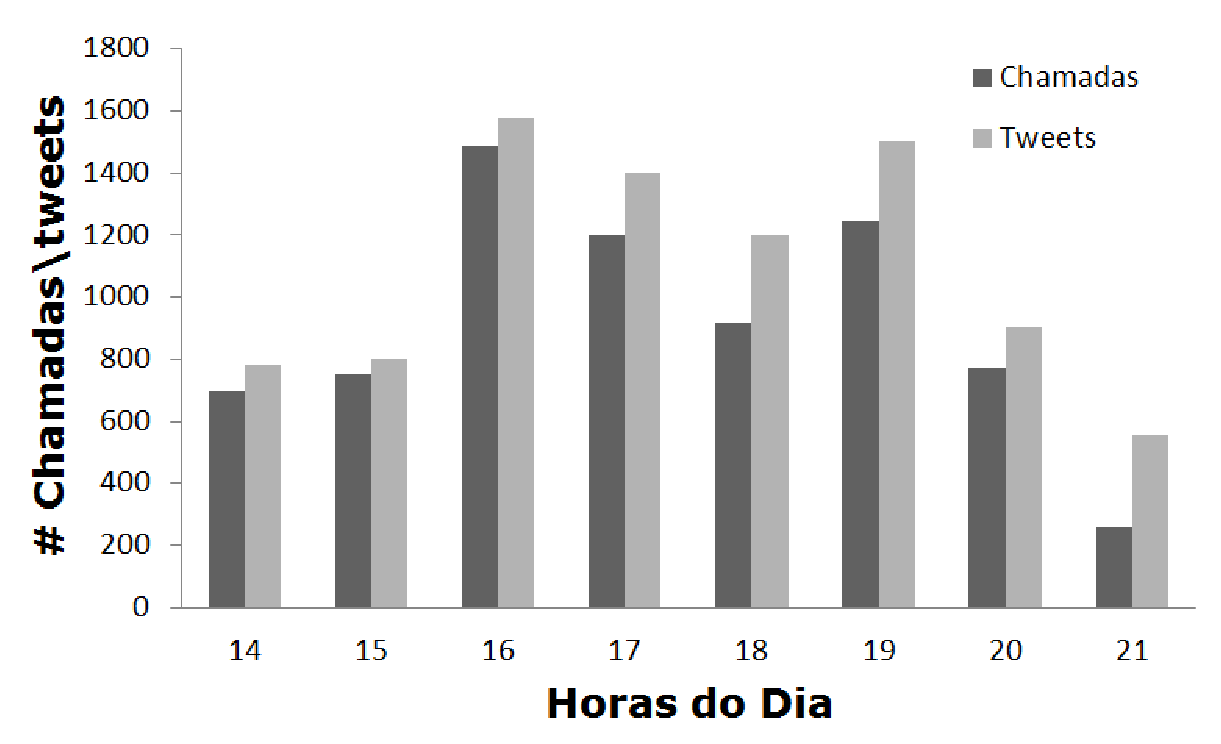
\includegraphics[width=0.5\linewidth]{Graficos/CallsTweets-Rio29-06-14.eps}
\caption{Quantidade de Chamadas/\textit{Tweets} por Hora - Rio de Janeiro 29/06/14}
\label{fig:qtdrio29a}
\end{figure}

\begin{figure}[ttt!]
\centering
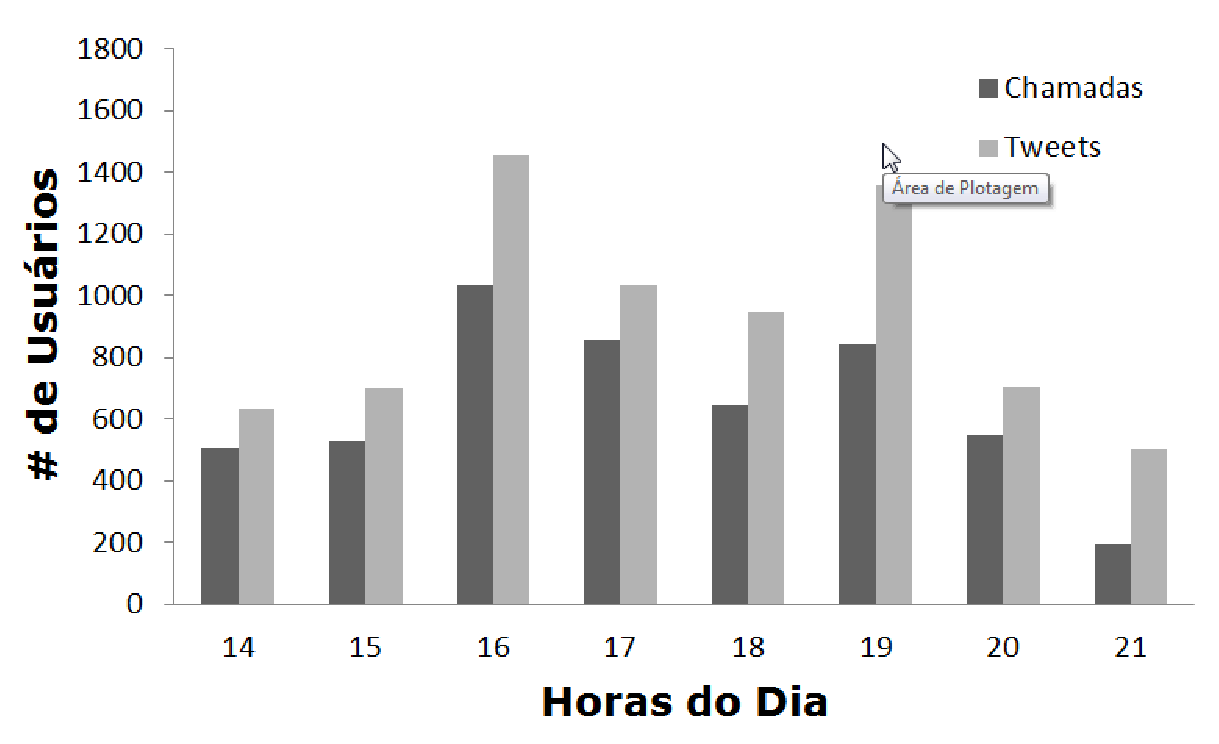
\includegraphics[width=0.5\linewidth]{Graficos/Users-Rio29-06-14.eps}
\caption{Quantidade de Usuários por Hora - Rio de Janeiro 29/06/14}
\label{fig:qtdrio29b}
\end{figure}




As Figuras \ref{fig:qtdrio29a} e \ref{fig:qtdrio29b} mostram os números de chamadas, {\it tweets} e usuários ao longo do tempo nas coleções do Rio de Janeiro (29/06/2014). Esta figura ilustra que o volume de dados disponível varia bastante segundo o horário de coleta, o que é esperado também para os padrões de movimentação das pessoas. Este resultado motiva a aplicação de modelos de predição específicos para diferentes períodos, conforme descrito na próxima seção.


\subsection{Avaliação}\label{subsec:methava}

%Cada modelo de previsão foi avaliado pela taxa de acerto das previsões em janelas de tempo $\Delta t$ iguais a 5 minutos.
%Para tal, cada coleção foi  subdividida em intervalos de uma hora. Dadas as variações nos volumes de dados observada (Figura \ref{fig:qtdrio29}), optou-se por desenvolver um modelo de predição para cada hora de forma a melhor capturar os padrões de locomoção em diferentes períodos. Em seguida, os dados de cada subcoleção foram divididos entre treino $\mathcal{D}$ e teste $\mathcal{T}$, conforme discutido na Seção \ref{subsec:modelagem}. Duas estratégias foram adotadas para fazer esta divisão.

Cada modelo de previsão foi avaliado em termos da taxa de acerto\footnote{A taxa de acerto é calculada como a fração de tuplas $<u_i,r_i,t>$ para as quais a previsão foi correta durante a fase de teste} das previsões em janelas de tempo $\Delta t$ iguais a 5 minutos.
Para tal, cada coleção foi  subdividida em intervalos de uma hora. Dadas as variações nos volumes de dados observadas  (Figura \ref{fig:qtdrio29a}), optou-se por desenvolver um modelo de predição para cada hora de forma a melhor capturar os padrões de locomoção em diferentes períodos. Em seguida, os dados de cada subcoleção foram divididos entre treino $\mathcal{D}$ e teste $\mathcal{T}$, conforme discutido na Seção \ref{subsec:modelagem}. Duas estratégias foram adotadas para fazer esta divisão, como descrito a seguir.

Para as coleções do Rio de Janeiro, como ambas cobrem o mesmo período no mesmo dia de semanas diferentes, a coleção do dia 29/06/14 foi utilizada como treino para aprender os modelos de cada hora. Estes modelos foram avaliados nos períodos correspondentes da base do dia 13/07/2014 (teste). Esta estratégia é mostrada na Figura \ref{fig:treinotestea}. Para as demais coleções, como não temos acesso a dados de múltiplos dias cobrindo o mesmo período,  foi adotada uma estratégia diferente. Cada hora no intervalo de tempo coberto pela coleção foi dividida em dois períodos de meia hora. O primeiro período foi utilizado para aprender o modelo (treino), e o segundo para avaliá-lo (teste). Esta estratégia é ilustrada na Figura \ref{fig:treinotesteb}.

  
\begin{figure}[ttt!]
\centering
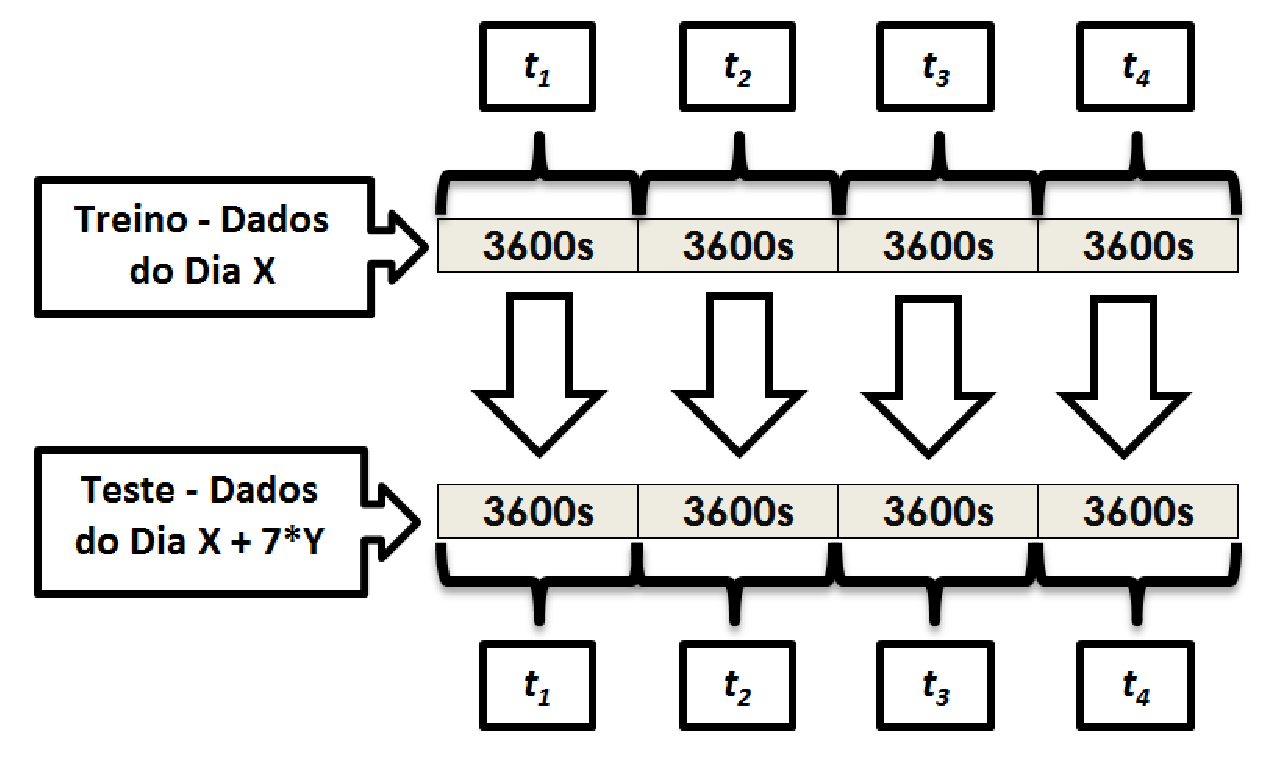
\includegraphics[width=0.5\linewidth]{Graficos/treinoteste2dias.eps}
\caption{Separação dos dados em Treino e Teste - Utilizando Dois Dias}
\label{fig:treinotestea}
\end{figure}

\begin{figure}[ttt!]
\centering
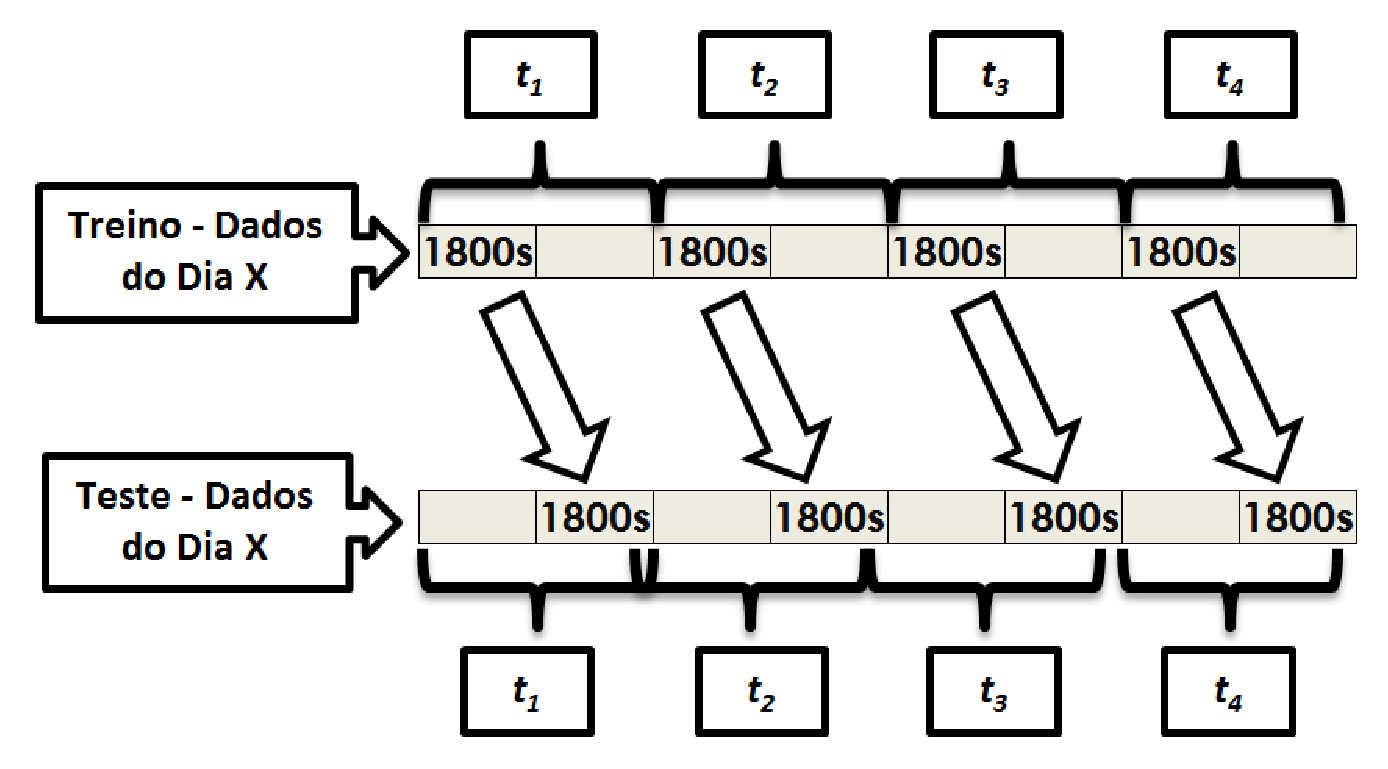
\includegraphics[width=0.5\linewidth]{Graficos/treinoteste1dia.eps}
\caption{Separação dos dados em Treino e Teste - Utilizando Um Dia}
\label{fig:treinotesteb}
\end{figure}

Para cada coleção, cada modelo de mobilidade foi avaliado usando, como conjuntos de treino e teste, somente  as chamadas, somente os \textit{tweets} e tanto chamadas quanto {\it tweets}. O objetivo do último cenário é avaliar o desempenho dos  modelos quando configurados com dados heterogêneos. A melhor forma de combinar  os dados das duas fontes não é óbvia já que modelos diferentes podem ter desempenhos relativos diferentes, dependendo do dado de entrada. Assim, nós consideramos e avaliamos duas estratégias: 

\begin{itemize}
	\item Associação de \textit{tweets} a chamadas: cada \textit{tweet} é associado à antena mais próxima de sua localização.
	\item Associação de chamadas a \textit{tweets}: cada antena da coleção de chamadas é considerado um ponto na região de simulação.   
\end{itemize}

Um aspecto importante da avaliação é a definição das regiões $R$ de cada modelo. Para as chamadas, o Leap Graph e o SMOOTH  consideram a localização de cada antena que aparece no conjunto $\mathcal{D}$ como uma região $r_{i}$. Porém no caso do SMOOTH,   novas regiões podem surgir durante o treino, de acordo com a movimentação dos usuários. Para os {\it tweets}, o SMOOTH considera inicialmente cada localização distinta associada a um  {\it tweet} em $\mathcal{D}$ como uma  região\footnote{Como descrito na Seção \ref{subsub:smooth}, cada região é definida no SMOOTH por um ponto, e a associação de um usuário a uma região é feita verificando um raio de cobertura $d$ a partir do {\it usuário}.},  e novas regiões podem surgir durante o treino. Para o Leap Graph,  os {\it tweets} foram agrupados em regiões circulares (com raio $d$) considerando suas localizações, e estas regiões foram inseridas em $R$. Para os dados combinados, foram adotadas as mesmas abordagens dependendo da estratégia de combinação feita. Já o MobDatU sempre divide a  área total de cada cidade em regiões quadrangulares não sobrepostas (Seção \ref{subsec:mobdatu}),  independentemente do tipo de dado.

%Em todos os casos, consideramos a distância $d$ que define cada região (e é usada na filtragem de dados) como 500 metros. Este valor, que representa o raio de cobertura de uma antena,  foi escolhido para que os resultados dos vários cenários  sejam comparáveis\footnote{Note que   as áreas das regiões do SMOOTH e do Leap Graph ($\pi d^2$) são maiores que as áreas das regiões definidas pelo MobDatU ($d^2$). Logo a nossa avaliação favorece os modelos de referência, uma vez que as predições são mais difíceis para regiões com áreas menores.}.   

Em todos os casos, consideramos a distância $d$ que define cada região como 500 metros. Este valor foi escolhido para que os resultados dos vários cenários pudessem ser comparados\footnote{Note que   as áreas das regiões do SMOOTH e do Leap Graph ($\pi d^2$) são maiores que as áreas das regiões definidas pelo MobDatU ($d^2$). Logo a nossa avaliação favorece os modelos de referência, uma vez que as predições são mais difíceis para regiões com áreas menores.}, uma vez que, para os dados de telefonia móvel, a posição geográfica informada tem granularidade dada pelo raio de cobertura de uma antena, a saber 500 metros . 
 


\section{Experimentos}\label{sec:experimentos}


Nossos resultados são sumarizados na Tabela \ref{tab:taxa} que apresenta, para cada cenário e para cada coleção de dados, os valores de taxa de acerto mínimo, máximo e médio considerando todos os intervalos de tempo $\Delta t = 5$ minutos em todas as horas do período de cada coleção. No geral, nota-se que cada modelo de referência funciona melhor se configurado para as fontes de dados homogêneas no qual ele foi avaliado anteriormente: o Leap Graph consegue taxa de acertos melhores quando utiliza somente chamadas, e o SMOOTH consegue resultados melhores quando utiliza somente \textit{tweets}. 

\begin{table}[httt!]
%\scriptsize
\centering
\caption{Taxa de Acerto dos Modelos de Previsão de Mobilidade}
\label{tab:taxa} 
\begin{tabular}{|c|p{1.0cm}|p{1.0cm}|p{1.0cm}|p{1.0cm}|p{1.0cm}|p{1.0cm}|p{1.0cm}|p{1.0cm}|} 
\cline{1-9} 
\multicolumn{9}{|c|}{Rio de Janeiro} \\ \hline
& \multicolumn{4}{|c|}{Chamadas} & \multicolumn{4}{|c|}{Tweets}  \\
\cline{2-9} 
Modelo & Mínimo & Máximo & Média & Desvio Padrão & Mínimo & Máximo & Média & Desvio Padrão\\
\hline
\multicolumn{1}{|l|}{SMOOTH} & 18\% & 55\% & 36,75\% & 0,13 & 34\% & 73\% & 52,12\% & 0,138 \\
\multicolumn{1}{|l|}{Leap Graph} & 68\% & 88\% & 78,13\% & 0,072 & 21\% & 60\% & 44,75\% & 0,129\\
\multicolumn{1}{|1|}{MobDatU} & 70\% & 87\% & 79,88\% & 0,063 & 37\% & 77\% & 55\% & 0,143\\ 
\cline{1-9} 
& \multicolumn{4}{|c|}{\textit{Tweets} a Chamadas} & \multicolumn{4}{|c|}{Chamadas a \textit{Tweets}} \\
\cline{2-9} 
Modelo & Mínimo & Máximo & Média & Desvio Padrão & Mínimo & Máximo & Média & Desvio Padrão\\
\hline
\multicolumn{1}{|l|}{SMOOTH} & 45\% & 52\% & 48\% & 0,26 & 38\% & 77\% & 51,5\% & 0,13\\
\multicolumn{1}{|l|}{Leap Graph} & 65\% & 84\% & 73,75\% & 0,062 & 25\% & 58\% & 41,63\% & 0,12\\
\multicolumn{1}{|1|}{MobDatU} & 67\% & 85\% & 74,38\% & 0,059 & 40\% & 79\% & 53,12\% & 0,129\\ 
\cline{1-9}
\hline
\multicolumn{9}{|c|}{Belo Horizonte 02/03/2013} \\ \hline
& \multicolumn{4}{|c|}{Chamadas} & \multicolumn{4}{|c|}{\textit{Tweets}}  \\
\cline{2-9} 
Modelo & Mínimo & Máximo & Média & Desvio Padrão & Mínimo & Máximo & Média & Desvio Padrão\\
\hline
\multicolumn{1}{|l|}{SMOOTH} & 20\% & 48\% & 35,37\% & 0,104 & 34\% & 70\% & 51,25\% & 0,125 \\
\multicolumn{1}{|l|}{Leap Graph} & 68\% & 80\% & 73\% & 0,044 & 21\% & 50\% & 40,75\% & 0,097 \\
\multicolumn{1}{|1|}{MobDatU} & 67\% & 82\% & 75,12\% & 0,047 & 37\% & 77\% & 54,5\% & 0,144\\ 
\cline{1-9} 
& \multicolumn{4}{|c|}{\textit{Tweets} a Chamadas} & \multicolumn{4}{|c|}{Chamadas a \textit{Tweets}} \\
\cline{2-9} 
Modelo & Mínimo & Máximo & Média & Desvio Padrão & Mínimo & Máximo & Média & Desvio Padrão \\
\hline
\multicolumn{1}{|l|}{SMOOTH} & 20\% & 35\% & 28,37\% & 0,053 & 38\% & 73\% & 50,85\% & 0,117\\
\multicolumn{1}{|l|}{Leap Graph} & 62\% & 77\% & 67,75\% & 0,054 & 30\% & 50\% & 36,75\% & 0,07\\
\multicolumn{1}{|1|}{MobDatU} & 58\% & 78\% & 66,87\% & 0,071 & 37\% & 77\% & 52,37\% & 0,131\\ 
\cline{1-9}
\hline
\multicolumn{9}{|c|}{Belo Horizonte 11/09/2013} \\ \hline
& \multicolumn{4}{|c|}{Chamadas} & \multicolumn{4}{|c|}{\textit{Tweets}} \\
\cline{2-9} 
Modelo & Mínimo & Máximo & Média & Desvio Padrão & Mínimo & Máximo & Média & Desvio Padrão \\
\hline
\multicolumn{1}{|l|}{SMOOTH} & 18\% & 40\% & 27,25\% & 0,08 & 38\% & 77\% & 53,25\% & 0,130 \\
\multicolumn{1}{|l|}{Leap Graph} & 67\%  & 75\% & 72,25\% & 0,025 & 22\% & 50\% & 36,5\% & 0,092\\
\multicolumn{1}{|1|}{MobDatU} & 70\% & 81\% & 73,75\% & 0,043 & 43\% & 78\% & 55,13\% & 0,128\\ 
\cline{1-9} 
& \multicolumn{4}{|c|}{\textit{Tweets} a Chamadas} & \multicolumn{4}{|c|}{Chamadas a \textit{Tweets}}  \\
\cline{2-9} 
Modelo & Mínimo & Máximo & Média & Desvio Padrão & Mínimo & Máximo & Média & Desvio Padrão \\
\hline
\multicolumn{1}{|l|}{SMOOTH} & 18\% & 32\% & 25,75\% & 0,051 & 42\% & 78\% & 57,62 & 0,138 \\
\multicolumn{1}{|l|}{Leap Graph} & 67\% & 86\% & 76,13\% & 0,063 & 22\% & 67\% & 41,75\% & 0,152\\
\multicolumn{1}{|1|}{MobDatU} & 67\% & 87\% & 75\% & 0,067 & 42\% & 80\% & 57,87 & 0,14\\ 
\cline{1-9}
\hline
\multicolumn{9}{|c|}{Recife} \\ \hline
& \multicolumn{4}{|c|}{Chamadas}  & \multicolumn{4}{|c|}{\textit{Tweets}} \\
\cline{2-9} 
Modelo & Mínimo & Máximo & Média & Desvio Padrão & Mínimo & Máximo & Média & Desvio Padrão \\
\hline
\multicolumn{1}{|l|}{SMOOTH} & 20\% & 35\% & 27,25\% & 0,053 & 42\% & 78\% & 43,12 & 0,139 \\
\multicolumn{1}{|l|}{Leap Graph} & 67\% & 86\% & 75,75 & 0,062 & 25\% & 67\% & 43,12\% & 0,139\\
\multicolumn{1}{|1|}{MobDatU} & 67\% & 87\% & 75\% & 0,067 & 42\% & 80\% & 57,87\% & 0,140\\ 
\cline{1-9} 
& \multicolumn{4}{|c|}{\textit{Tweets} a Chamadas} & \multicolumn{4}{|c|}{Chamadas a \textit{Tweets}} \\
\cline{2-9} 
Modelo & Mínimo & Máximo & Média & Desvio Padrão & Mínimo & Máximo & Média & Desvio Padrão \\
\hline
\multicolumn{1}{|l|}{SMOOTH} & 19\% & 34\% & 26,13\% & 0,061 & 42\% & 77\% & 53,38\% & 0,121 \\
\multicolumn{1}{|l|}{Leap Graph} & 69\% & 75\% & 72,12\% & 0,023 & 22\% & 45\% & 35,13\% & 0,075\\
\multicolumn{1}{|1|}{MobDatU} & 70\% & 77\% & 73\% & 0,031 & 43\% & 78\% & 54,63\% & 0,124\\ 
\cline{1-9}
\hline
\multicolumn{9}{|c|}{Fortaleza} \\ \hline
& \multicolumn{4}{|c|}{Chamadas} & \multicolumn{4}{|c|}{\textit{Tweets}} \\
\cline{2-9} 
Modelo & Mínimo & Máximo & Média & Desvio Padrão & Mínimo & Máximo & Média & Desvio Padrão \\
\hline
\multicolumn{1}{|l|}{SMOOTH} & 18\% & 35\% & 26,25\% & 0,062 & 40\% & 77\% & 56,63\% & 0,138\\
\multicolumn{1}{|l|}{Leap Graph} & 65\% & 84\% & 73,75\% & 0,063 & 25\% & 67\% & 42,75\% & 0,140\\
\multicolumn{1}{|1|}{MobDatU} & 67\% & 85\% & 74,37\% & 0,059 & 42\% & 80\% & 57,87\% & 0,14\\ 
\cline{1-9} 
& \multicolumn{4}{|c|}{\textit{Tweets} a Chamadas} & \multicolumn{4}{|c|}{Chamadas a \textit{Tweets}}  \\
\cline{2-9} 
Modelo & Mínimo & Máximo & Média & Desvio Padrão & Mínimo & Máximo & Média & Desvio Padrão \\
\hline
\multicolumn{1}{|l|}{SMOOTH} & 22\% & 37\% & 28,75\% & 0,053 & 42\% & 77\% & 52,12\% & 0,118 \\
\multicolumn{1}{|l|}{Leap Graph} & 62\% & 75\% & 66,87\% & 0,039 & 30\% & 50\% & 37,63\% & 0,078\\
\multicolumn{1}{|1|}{MobDatU} & 56\% & 78\% & 67,37\% & 0,072 & 38\% & 79\% & 52,25\% & 0,129\\ 
\cline{1-9}
\hline
\end{tabular}
\end{table}

Por exemplo, considerando  a coleção de dados do Rio de Janeiro, nota-se que,  quando os dados de chamadas são usados como entrada,  o SMOOTH tem um desempenho médio degradado de 53\% em relação ao Leap Graph. Já quando são usados os \textit{tweets}, o Leap Graph possui um desempenho de 14\% pior que o SMOOTH. Quanto aos cenários com dados heterogêneos, a taxa de acerto de cada modelo foi um pouco menor em relação ao  seu melhor cenário.  Ou seja, os modelos de referência se comportam um pouco pior em cenários com dados heterogêneos.  

Em contrapartida, o MobDatU tem um desempenho comparável aos melhores resultados dos modelos de referência em todos os cenários. Para o cenário de chamadas, ele tem uma taxa de acerto ligeiramente maior que a do Leap Graph e muito superior (109\%) à do SMOOTH. Já para o cenário de \textit{tweets}, os resultados do Leap Graph são piores em 19\% quando comparados aos do MobDatU, enquanto o SMOOTH consegue resultados bem próximos aos do nosso modelo. Comparando os dois cenários com dados homogêneos, nota-se que o MobDatU tem uma taxa de acerto bem maior  no cenário de chamadas. A razão para este resultado é um maior número de regiões distintas presentes somente no conjunto de teste para os dados de {\it tweets}. Regiões que não aparecem no conjunto de treino terão popularidade e taxas de transição nulas no modelo e nunca serão previstas. Logo, regiões que só aparecem no teste necessariamente levam a previsões erradas do modelo\footnote{ Note que este maior número de regiões novas no teste foi observada em todas coleções, a despeito das diferenças de volumes de dados de chamadas e {\it tweets} discutidos na Seção \ref{sec:dados}.}.

Em relação ao cenário com dados heterogêneos, assim como os modelos de referência, o MobDatU apresenta um desempenho um pouco pior em relação aos cenários de dados homogêneos, mas ainda superior, em média, ao dos modelos de referência.
Quanto às  estratégias de combinação de dados, observa-se que cada  modelo de referência teve melhor desempenho quando a estratégia adotada faz a associação tendo como alvo o tipo de dado para o qual o modelo tem melhor precisão (chamadas para o Leap Graph e para o MobDatU, {\it tweets} para o SMOOTH).  

Os resultados obtidos para as outras coleções de dados apresentam um comportamento similar aos dados do Rio de Janeiro. Uma exceção ocorre na coleção de Belo Horizonte (11/09/2013), na qual   o MobDatU  teve resultados melhores nos cenários com dados heterogêneos. 
Vale ressaltar que o uso de dados heterogêneos viabiliza uma realização de previsões para um número  de usuários (isto é cobertura de usuários) potencialmente muito maior\footnote{Já que as coleções de chamadas e \textit{tweets} não apresentam nenhum parâmetro que indicasse a existência de um mesmo usuário em ambas as fontes, foi considerado que os usuários dos dados de chamadas eram diferentes dos de \textit{tweets} conforme descrito na Seção \ref{sec:dados}.}, o que pode compensar eventuais perdas nas taxas de acerto quando comparadas às obtidas  com dados homogêneos.


As Figuras \ref{fig:taxadeacertorioa}, \ref{fig:taxadeacertoriob} e \ref{fig:taxadeacertorioc} mostram as taxas de acerto de cada modelo ao longo do período coberto pela coleção do Rio de Janeiro para os cenários com dados homogêneos e para um cenário com dado heterogêneo. Comparando esta figura com a Figura \ref{fig:qtdrio29a}, nota-se que as maiores taxas de acertos foram obtidas em períodos com maior o volume de dados, o que era esperado. A figura também mostra que os ganhos do MobDatU sobre o melhor modelo de referência podem ser maiores que os mostrados na Tabela \ref{tab:taxa}.  Por exemplo, na Figura \ref{fig:taxadeacertoriob}, para o intervalo de 16 horas, a taxa de acerto do MobDatU supera em 6\% a do SMOOTH (melhor modelo de referência), enquanto na Figura \ref{fig:taxadeacertorioa}, o MobDatU supera o Leap Graph em 5\% para o período de 20 horas. 
Resultados semelhantes foram observados também para as outras coleções.

\begin{figure}[!ttt]
\centering
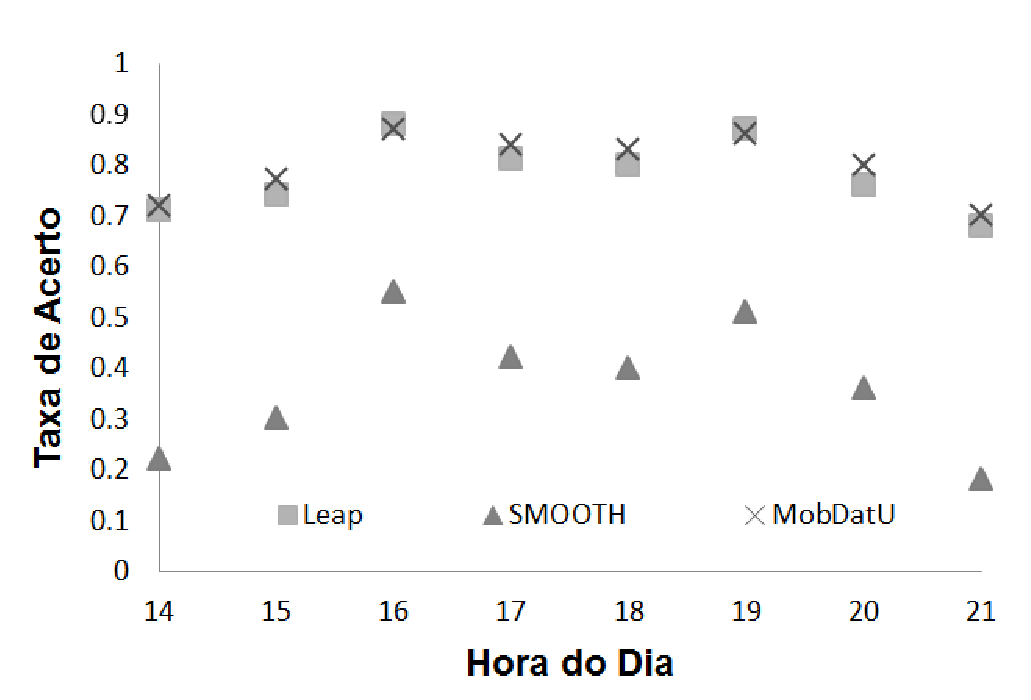
\includegraphics[width=0.5\linewidth]{Graficos/txchamadasRiohora.eps}
\caption{Taxa de Acerto para Cenários 1, 2 e 3 de Chamadas - Rio de Janeiro}
\label{fig:taxadeacertorioa}
\end{figure}

\begin{figure}[!ttt]
\centering
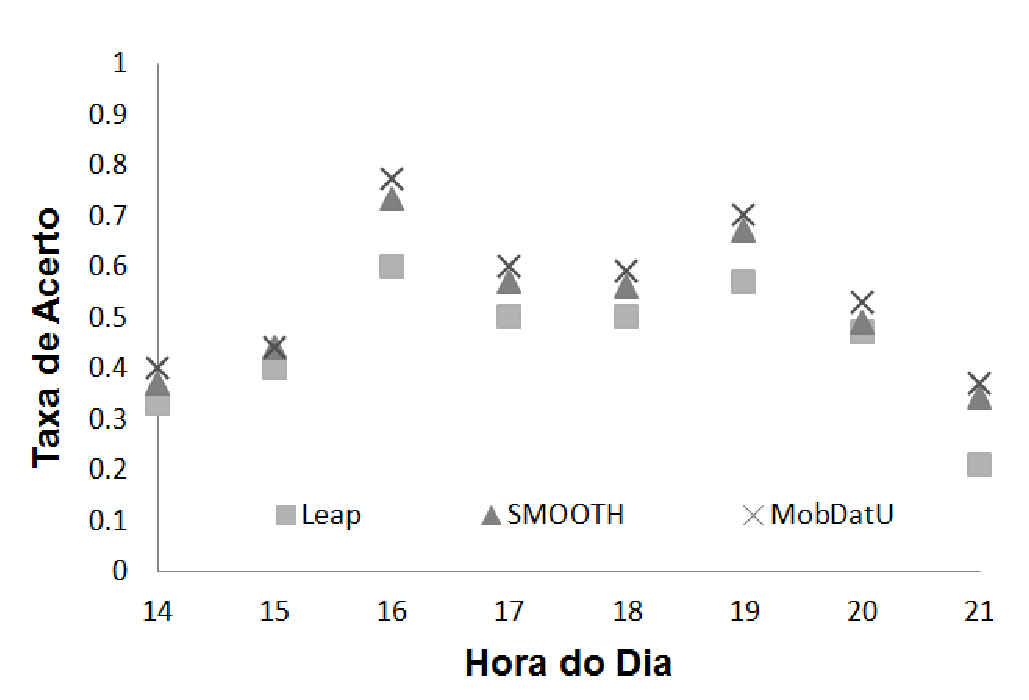
\includegraphics[width=0.5\linewidth]{Graficos/txtweetRiohora.eps}
\caption{Taxa de Acerto para Cenários 1, 2 e 3 de \textit{Tweets}- Rio de Janeiro}
\label{fig:taxadeacertoriob}
\end{figure}

\begin{figure}[!ttt]
\centering
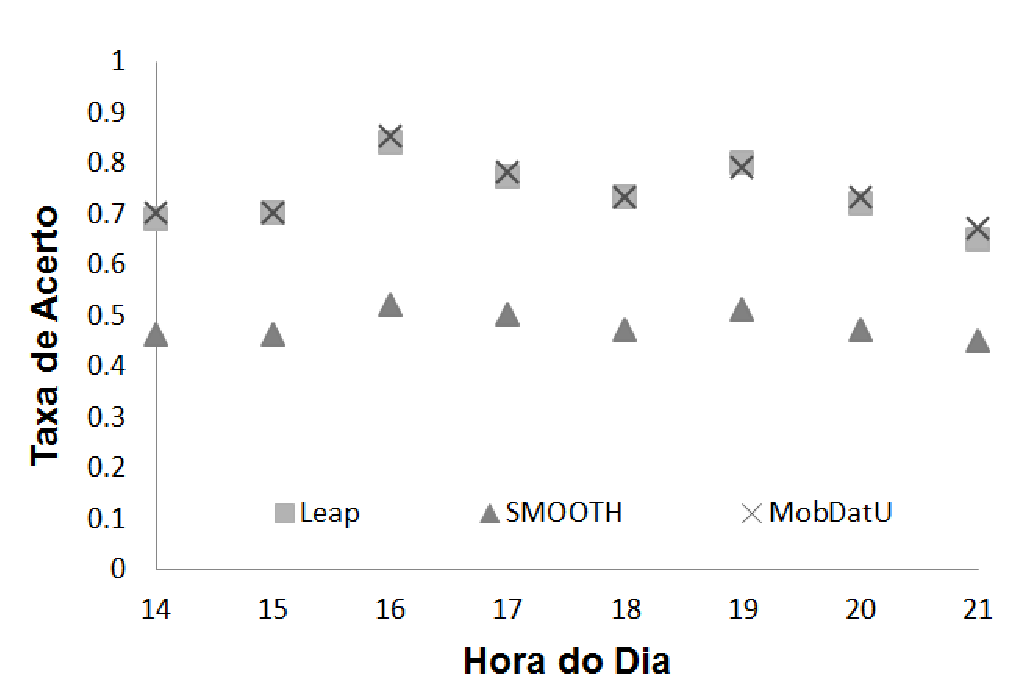
\includegraphics[width=0.5\linewidth]{Graficos/txtwittercchamadaRiohora.eps}
\caption{Taxa de Acerto para Cenários 1, 2 e 3 de \textit{Tweets} para Chamadas - Rio de Janeiro}
\label{fig:taxadeacertorioc}
\end{figure}

%Em suma, o MobDatU mostrou ser um modelo mais robusto, conseguindo desempenho comparável (e por vezes superior) ao do melhor modelo de referência, em todos os cenários com dados homogêneos e heterogêneos.  Em contrapartida, tanto SMOOTH quanto Leap Graph podem ter grande perda de desempenho, dependendo do tipo de dado de entrada. A superioridade do nosso modelo pode ser explicada por ele considerar tanto a popularidade das regiões quanto a frequência de transições entre as regiões. Ambos os aspectos são fatores importantes que influenciam como as pessoas se movimentam em uma cidade. Além disto, como estes aspectos podem ser capturados tanto pelas chamadas telefônicas realizadas quanto pelos {\it tweets} compartilhados, o MobDatU se adéqua bem a ambos tipos de dados.

Em suma, o MobDatU mostrou se adequar bem a dados distintos, conseguindo desempenho comparável (e por vezes superior) ao do melhor modelo de referência, em todos os cenários com dados homogêneos e heterogêneos.  Em contrapartida, tanto SMOOTH quanto Leap Graph podem ter grande perda de desempenho, dependendo do tipo de dado de entrada. A superioridade do nosso modelo pode ser explicada por ele considerar tanto a popularidade das regiões quanto a frequência de transições entre as regiões. Ambos os aspectos são fatores importantes que influenciam como as pessoas se movimentam em uma cidade. Além disto, como estes aspectos podem ser capturados tanto pelas chamadas telefônicas realizadas quanto pelos {\it tweets} compartilhados, o MobDatU mostrou um bom funcionamento para ambos os tipos de dados.




\section {Conclusão e Trabalhos Futuros}\label{sec:conclusao}

%Neste artigo, foi proposto um novo modelo de previsão de mobilidade humana, o MobDatU. O modelo proposto, assim como dois modelos estado-da-arte, foram avaliados em diversos cenários com dados reais homogêneos e heterogêneos. Os experimentos indicaram que nenhum dos dois modelos de referência é superior em todos os cenários investigados, o que demonstra a sensibilidade dos mesmos aos dados disponíveis. Já o MobDatU se mostrou um modelo muito robusto, sendo  pelo menos comparável (e por vezes superior) ao melhor modelo de referência em todos os cenários. Também foi mostrado que o volume de dados, tanto de chamadas telefônicas quanto de {\it tweets}, varia bastante durante o dia, o que afeta a precisão de todos os modelos. Logo, a diferença do volume de dados por período de tempo é algo importante a se considerar quando for realizar a previsão da mobilidade humana.

Neste artigo, foi proposto um novo modelo de previsão de mobilidade humana, o MobDatU. O modelo proposto, assim como dois modelos estado-da-arte, foram avaliados em diversos cenários com dados reais homogêneos e heterogêneos. Os experimentos indicaram que nenhum dos dois modelos de referência é superior em todos os cenários investigados, o que demonstra a sensibilidade dos mesmos aos dados disponíveis. Já o MobDatU se adequou bem a ambos tipos de dados, sendo  pelo menos comparável (e por vezes superior) ao melhor modelo de referência em todos os cenários. Também foi mostrado que o volume de dados, tanto de chamadas telefônicas quanto de {\it tweets}, varia bastante durante o dia, o que afeta a precisão de todos os modelos. Logo, a diferença do volume de dados por período de tempo é algo importante a se considerar quando for realizar a previsão da mobilidade humana.

Como trabalho futuro pretende-se investigar novas estratégias de combinação de dados heterogêneos que permitam a identificação (ou pelo menos a inferência da presença) de um mesmo usuário em múltiplas coleções. Este
é um grande desafio técnico uma vez que essas coleções tipicamente são obtidas de forma independente. Pretende-se também adaptar o MobDatU para prever o volume de pessoas que estarão em uma determinada região em um certo período. Tais previsões são úteis para suportar decisões de gerenciamento e planejamento urbano.


% An example of a floating figure using the graphicx package.
% Note that \label must occur AFTER (or within) \caption.
% For figures, \caption should occur after the \includegraphics.
% Note that IEEEtran v1.7 and later has special internal code that
% is designed to preserve the operation of \label within \caption
% even when the captionsoff option is in effect. However, because
% of issues like this, it may be the safest practice to put all your
% \label just after \caption rather than within \caption{}.
%
% Reminder: the "draftcls" or "draftclsnofoot", not "draft", class
% option should be used if it is desired that the figures are to be
% displayed while in draft mode.
%
%\begin{figure}[!t]
%\centering
%\includegraphics[width=2.5in]{myfigure}
% where an .eps filename suffix will be assumed under latex, 
% and a .pdf suffix will be assumed for pdflatex; or what has been declared
% via \DeclareGraphicsExtensions.
%\caption{Simulation Results}
%\label{fig_sim}
%\end{figure}

% Note that IEEE typically puts floats only at the top, even when this
% results in a large percentage of a column being occupied by floats.


% An example of a double column floating figure using two subfigures.
% (The subfig.sty package must be loaded for this to work.)
% The subfigure \label commands are set within each subfloat command, the
% \label for the overall figure must come after \caption.
% \hfil must be used as a separator to get equal spacing.
% The subfigure.sty package works much the same way, except \subfigure is
% used instead of \subfloat.
%
%\begin{figure*}[!t]
%\centerline{\subfloat[Case I]\includegraphics[width=2.5in]{subfigcase1}%
%\label{fig_first_case}}
%\hfil
%\subfloat[Case II]{\includegraphics[width=2.5in]{subfigcase2}%
%\label{fig_second_case}}}
%\caption{Simulation results}
%\label{fig_sim}
%\end{figure*}
%
% Note that often IEEE papers with subfigures do not employ subfigure
% captions (using the optional argument to \subfloat), but instead will
% reference/describe all of them (a), (b), etc., within the main caption.


% An example of a floating table. Note that, for IEEE style tables, the 
% \caption command should come BEFORE the table. Table text will default to
% \footnotesize as IEEE normally uses this smaller font for tables.
% The \label must come after \caption as always.
%
%\begin{table}[!t]
%% increase table row spacing, adjust to taste
%\renewcommand{\arraystretch}{1.3}
% if using array.sty, it might be a good idea to tweak the value of
% \extrarowheight as needed to properly center the text within the cells
%\caption{An Example of a Table}
%\label{table_example}
%\centering
%% Some packages, such as MDW tools, offer better commands for making tables
%% than the plain LaTeX2e tabular which is used here.
%\begin{tabular}{|c||c|}
%\hline
%One & Two\\
%\hline
%Three & Four\\
%\hline
%\end{tabular}
%\end{table}


% Note that IEEE does not put floats in the very first column - or typically
% anywhere on the first page for that matter. Also, in-text middle ("here")
% positioning is not used. Most IEEE journals/conferences use top floats
% exclusively. Note that, LaTeX2e, unlike IEEE journals/conferences, places
% footnotes above bottom floats. This can be corrected via the \fnbelowfloat
% command of the stfloats package.





% use section* for acknowledgement
\section*{Agradecimentos}

Os autores agradecem o apoio do INCTWeb (MCT/CNPq 573871/2008-6), CNPq, CAPES, FAPEMIG e FAPERJ.


% trigger a \newpage just before the given reference
% number - used to balance the columns on the last page
% adjust value as needed - may need to be readjusted if
% the document is modified later
%\IEEEtriggeratref{8}
% The "triggered" command can be changed if desired:
%\IEEEtriggercmd{\enlargethispage{-5in}}

% references section

% can use a bibliography generated by BibTeX as a .bbl file
% BibTeX documentation can be easily obtained at:
% http://www.ctan.org/tex-archive/biblio/bibtex/contrib/doc/
% The IEEEtran BibTeX style support page is at:
% http://www.michaelshell.org/tex/ieeetran/bibtex/
%\bibliographystyle{IEEEtran}
% argument is your BibTeX string definitions and bibliography database(s)
%\bibliography{IEEEabrv,../bib/paper}
%
% <OR> manually copy in the resultant .bbl file
% set second argument of \begin to the number of references
% (used to reserve space for the reference number labels box)
\bibliographystyle{IEEEtran}
\bibliography{bibfile}



% that's all folks
\end{document}


